\documentclass[12pt,a4paper,oneside]{ctexart}
\usepackage{amsmath,amsthm,amssymb,wrapfig,graphicx,float,tabularx}
\title{切变模量实验报告}
\author{张博厚 PB22071354}
\date{2023.6.12}
\begin{document}
\maketitle
\tableofcontents
\newpage
\section{实验背景与目的}
切变模量,又称剪切模量/刚性模量,材料的力学性能指标之一,是指材料在剪切应力作用下,
在弹性变形比例极限范围内,切应力与切应变的比值.切变模量表征材料抵抗切应变的能力,模量大,则表示材料的刚性强.本实验中
采用扭摆实验装置来测量金属丝的切变模量,尽量避免测量较难测准的物理量,提高实验精度.
\section{实验原理}
本实验的实验对象是一根上下均匀而细长的钢丝,在几何上可认为是一个半径为
$R$,长度为$L$的细长圆柱体.将钢丝上端固定,下端面发生扭转,则在弹性限度内有
\begin{equation}
    \tau = G\gamma
\end{equation}
式中$G$即为材料的切变模量,如下图所示:
\begin{figure}[H]
    \centering
    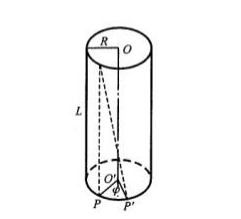
\includegraphics[scale=1.2]{扭转形变示意图.png}
    \caption{金属丝扭转形变示意图}
\end{figure}
设钢丝下端面绕中轴线转过的角度为$\phi$(图中P点转到P'点),根据位错理论,
金属丝各截面均相应地发生了转动,其单位长度的转角$\frac{d\phi}{dl}=\frac{\phi}{L}$,
选取其中长为$dl$的体积元,可以推知在其中半径为$\rho$的位置,切应变为
\begin{equation}
    \gamma_{\rho}=\rho\dfrac{d\phi}{dl}
\end{equation}
其产生的恢复力矩
\begin{equation}
    dM=\tau_{\rho}\cdot\rho\cdot2\pi\rho\cdot d\rho=2\pi G\rho^3\dfrac{d\phi}{dl}\cdot d\rho
\end{equation}
故总力矩为
\begin{equation}
    M=\int_0^R2\pi G\rho^3\dfrac{d\phi}{dl}\cdot d\rho=\dfrac{\pi}{2}GR^4\dfrac{d\phi}{dl}=\dfrac{\pi}{2}GR^4\dfrac{\phi}{L}
\end{equation}
为求出钢丝的恢复力矩,在其下端悬挂一圆盘,可绕中轴线自由扭动,则摆扭过的角度正比于所受的扭力矩:
\begin{equation}
    M=D\phi
\end{equation}
又由转动定律,
\begin{equation}
    M=I_0\dfrac{d^2\phi}{dt^2}
\end{equation}
联立(5)(6),得
\begin{equation}
    \dfrac{d^2\phi}{dt^2}+\dfrac{D}{I_0}\phi=0
\end{equation}
这是一个简谐运动微分方程,其周期为
\begin{equation}
    T_0=2\pi\sqrt{\dfrac{I_0}{D}}
\end{equation}
但作为扭摆的圆盘上有一个夹具,并不对称,直接计算$I_0$比较困难,因此可将
一个金属环对称地置于圆盘上.设环的质量为$m$,内外半径分别为$r_1,r_2$,易知其转动惯量为
$I_1=\frac{1}{2}m(r_1^2+r_2^2)$,则此时扭摆周期为
\begin{equation}
    T_1=2\pi\sqrt{\dfrac{I_0+I_1}{D}}
\end{equation}
联立(4)(5)(6)(8)(9),得
\begin{equation}
    D=\dfrac{2\pi^2m(r_1^2+r_2^2)}{T_1^2-T_0^2}
\end{equation}
\begin{equation}
    G=\dfrac{4\pi Lm(r_1^2+r_2^2)}{R^4(T_1^2-T_0^2)}
\end{equation}
\section{实验内容}
\subsection{实验仪器}
扭摆装置,螺旋测微器,游标卡尺,米尺,秒表
\subsection{实验步骤}\noindent
1. 调整扭摆装置,使钢丝与圆盘面垂直,圆环能方便地置于圆盘上.\\
2. 用螺旋测微器测量钢丝直径,用游标卡尺测量环的内外径,用米尺测量钢丝的有效长度.\\
3. 写出相对误差公式,据此估算应测量的周期数目.\\
4. 选定扭转角度,测量放置金属环前后多个周期的时长.\\
5. 计算钢丝的切变模量 G 和扭转模量 D,完成误差分析.\\
6. 测量不同扭转角度下的周期,研究钢丝的切变模量与其扭转角度的关系.
\subsection{方案设计}
在实验中,直接测量量为金属丝,金属环的直径,将式(11)改写为
\begin{equation}
    G=\dfrac{16\pi Lm(d_1^2+d_2^2)}{d^4(T_1^2-T_0^2)}
\end{equation}
根据最大不确定度公式,有
$$\dfrac{\Delta G}{G}=\dfrac{\Delta L}{L}+\dfrac{\Delta m}{m}
        +\dfrac{2d_1\Delta d_1}{d_1^2+d_2^2}+\dfrac{2d_2\Delta d_2}{d_1^2+d_2^2}
        +4\dfrac{\Delta d}{d}+\dfrac{2T_0\Delta t_0}{N_0(T_1^2-T_0^2)}+\dfrac{2T_1\Delta T_1}{N_1(T_1^2-T_0^2)}$$
粗侧数据及相应的实验设计见附录1:实验方案设计

\section{数据记录与处理}\noindent
原始数据见附录2:实验原始数据\\
考虑零点误差$d_0=-0.019mm$,钢丝直径d的平均值为
$$
\overline{d}=\frac{1}{n}\sum_{i=1}^{n}d_i=\frac{0.779+0.782+0.786+0.789+0.783+0.787}{6}\,\mathrm{mm}=0.78433\,\mathrm{mm}
$$
钢丝直径d的标准差
$$
\begin{aligned}
\sigma_{d}&=\sqrt{\frac{1}{n-1}\sum_{i=1}^n\left(d_i-\overline{d}\right)^2}=0.0036697\,\mathrm{mm}
\end{aligned}
$$
其A类不确定度为
$$\Delta_{A,d}=\dfrac{\sigma_{d}}{\sqrt{n}}=1.498\times10^{-3}mm$$
B类不确定度为
$$
\Delta_{B,d}=0.004\,\mathrm{mm}
$$
钢丝直径d的展伸不确定度
$$
\begin{aligned}
U_{d}&=\sqrt{\left(t_P\Delta_{A,d}\right)^2+\left(k_P\frac{\Delta_{B,d}}{C}\right)^2}\\
&=\sqrt{\left(2.57\times1.498\times10^{-3}\right)^2+\left(1.96\times\frac{0.004}{3}\right)^2}\,\mathrm{mm}\\
&=0.004653\,\mathrm{mm}\qquad(P=0.95)
\end{aligned}
$$
\noindent
环内直径
$$
d_1=79.62\,\mathrm{mm}
$$
其A类不确定度为$0$,B类不确定度为
$$
\Delta_{B,d1}=0.02\,\mathrm{mm}
$$
展伸不确定度为
$$
U_{d1}=k_P\frac{\Delta_{B,d1}}{C}=1.96\times\frac{0.02}{\sqrt{3}}\,\mathrm{mm}=0.022632\,\mathrm{mm}\qquad(P=0.95)
$$
\noindent
环外直径
$$
d_2=100.16\,\mathrm{mm}
$$
其A类不确定度为$0$,B类不确定度为
$$
\Delta_{B,d2}=0.02\,\mathrm{mm}
$$
展伸不确定度为
$$
U_{d2}=k_P\frac{\Delta_{B,d2}}{C}=1.96\times\frac{0.02}{\sqrt{3}}\,\mathrm{mm}=0.022632\,\mathrm{mm}\qquad(P=0.95)
$$
\noindent
钢丝长度
$$
L=48.3\,\mathrm{cm}
$$
B类不确定度
$$
\Delta_{B,L}=\sqrt{\Delta_\text{仪}^2+\Delta_\text{估}^2}=\sqrt{0.1^2+0.05^2}\,\mathrm{cm}=0.1118\,\mathrm{cm}
$$
展伸不确定度
$$
U_{L}=k_P\frac{\Delta_{B,L}}{C}=1.96\times\frac{0.1118}{3}\,\mathrm{cm}=0.073045\,\mathrm{cm},P=0.95
$$
\noindent
圆环质量
$$
m=478.4\,\mathrm{g}
$$
B类不确定度为(采用七级物理天平)
$$
\Delta_{B,m}=0.08\,\mathrm{g}
$$
展伸不确定度为
$$
U_{m}=k_P\frac{\Delta_{B,m}}{C}=1.96\times\frac{0.08}{3}\,\mathrm{g}=0.0523\,\mathrm{g}\qquad(P=0.95)
$$
\noindent
不带圆环时,$N_0=33$,所用时间的平均值
$$\overline{t_0}=\frac{1}{3}(83.58s+83.63s+83.64s)=83.62s$$
周期平均值
$$
\overline{T_0}=\frac{\overline{t_0}}{N_0}=2.5339\,\mathrm{s}
$$
$t_0$的标准差为
$$\sigma_{t_0}=\sqrt{\dfrac{(83.58-83.62)^2+(83.63-83.62)^2+(83.64-83.62)^2}{2}}=0.0324s$$
其A类不确定度为
$$\Delta_{A,t_0}=\dfrac{\sigma_{t_0}}{\sqrt{n}}=0.0187s$$
B类不确定度
$$
\Delta_{B,t0}=0.2\,\mathrm{s}
$$
展伸不确定度为
$$
U_{t0}=\sqrt{(2.57\times0.0187)^2+(1.96\times\frac{0.2}{3})^2}=0.1392s \qquad(P=0.95)
$$
带圆环时,$N_1=49$,所用时间的平均值
$$\overline{t_1}=\dfrac{1}{3}(184.39s+184.54s+184.89s)=184.61s$$
周期T1的平均值
$$
\overline{T_1}=\frac{\overline{t_1}}{N_1}\,\mathrm{s}=3.7676\,\mathrm{s}
$$
$t_1$的标准差为
$$\sigma_{t1}=\sqrt{\dfrac{(184.39-184.61)^2+(184.54-184.61)^2+(184.89-184.61)^2}{2}}=0.2566s$$
其A类不确定度为
$$\Delta_{A,t_1}=\dfrac{\sigma_{t1}}{\sqrt{n}}=0.1481s$$
B类不确定度
$$
\Delta_{B,t_1}=0.2\,\mathrm{s}
$$
展伸不确定度
$$
U_{t1}=\sqrt{(2.57\times0.1481)^2+(1.96\times\frac{0.2}{3})^2}=0.4024s \qquad(P=0.95)
$$
由式(10),改写得
\begin{equation}
    D=\dfrac{\pi^2m(d_1^2+d_2^2)}{2(T_1^2-T_0^2)}
\end{equation}
代入数据得,扭转模量
$$
D=\frac{\pi^2\times 0.4784 \left(0.07962^2+0.10016^2\right)}{2\times(3.7676^2-2.5339^2)}\,\mathrm{kg·m^2/s^2}=4.9719 \times 10^{-3}\,\mathrm{kg·m^2/s^2}
$$
展伸不确定度
$$
\dfrac{U_D}{D}=\sqrt{(\frac{U_m}{m})^2+(\frac{2d_1U_{d_1}}{d_1^2+d_2^2})^2+(\frac{2d_2U_{d_2}}{d_1^2+d_2^2})^2+(\frac{2T_1U_{t_1}}{N_1(T_1^2-T_0^2)})^2+(\frac{2T_0U_{t_0}}{N_0(T_1^2-T_0^2)})^2}
$$
得$$U_D=4\times10^{-5}kg\cdot m^2\cdot s^{-2} \qquad(P=0.95)$$
故
$$
D=\left(0.00497 \pm 0.00004\right)kg\cdot m^2\cdot s^{-2}
$$
\noindent
由式(12),切变模量
$$
G=\frac{16 \pi\times 0.483\times 0.4784 \left(0.07962^2+0.10016^2\right)}{0.00078433^4\times \left(3.7676^2-2.5339^2\right)}\,\mathrm{kg/(m·s^2)}=6.4635 \times 10^{10}\,\mathrm{kg/(m·s^2)}
$$
其展伸不确定度
\begin{footnotesize}
$$
\dfrac{U_G}{G}=\sqrt{(\frac{U_L}{L})^2+4(\frac{U_d}{d})^2+(\frac{U_m}{m})^2+(\frac{2d_1U_{d_1}}{d_1^2+d_2^2})^2+(\frac{2d_2U_{d_2}}{d_1^2+d_2^2})^2+(\frac{2T_1U_{t_1}}{N_1(T_1^2-T_0^2)})^2+(\frac{2T_0U_{t_0}}{N_0(T_1^2-T_0^2)})^2}
$$
\end{footnotesize}
得
$$U_G=2.8\times10^9kg/(m·s^2) \qquad(P=0.95)$$
故
$$
G=\left(6.46 \pm 0.28\right) \times 10^{10}\,\mathrm{kg/(m·s^2)}
$$
\section{思考与讨论}
\subsection{本题是否满足$\gamma<<1$的条件?}
    本题中扭转角度$\phi=270^{\circ}=4.712rad$,由式(2),知$$\gamma_{max}=\dfrac{\overline{d}}{2}\cdot\dfrac{\phi}{L}=3.826\times10^{-3}<<1$$
满足条件
\subsection{为提高精度,本实验在设计上做了哪些安排?实验中应注意什么?}
在设计上,本实验设法避免测量难以测量的物理量.由于圆盘的转动惯量难以计算和测量,利用
摆上放置圆盘前后的周期关系,将转动惯量这一难测量的量转化为测量金属环的质量与内外径,提高了实验精度;此外
在设计实验时,找到对结果影响最大的主要误差项,对其进行多次测量减小误差;测量多个周期的总时间,也减小了时间测量误差对结果的影响.
\par
在实验操作中,应注意规范使用千分尺,游标卡尺等实验仪器,避免出现读数错误;在测量前应调整扭摆装置,使得钢丝与圆盘面垂直;测量时应适当调整扭摆,
使之仅围绕其中轴线自转,避免其做圆锥摆运动.
\newpage
\section{附录}
\subsection{实验方案设计}
\subsection{实验原始数据}
\end{document}